% Options for packages loaded elsewhere
\PassOptionsToPackage{unicode}{hyperref}
\PassOptionsToPackage{hyphens}{url}
%
\documentclass[
]{book}
\usepackage{amsmath,amssymb}
\usepackage{lmodern}
\usepackage{ifxetex,ifluatex}
\ifnum 0\ifxetex 1\fi\ifluatex 1\fi=0 % if pdftex
  \usepackage[T1]{fontenc}
  \usepackage[utf8]{inputenc}
  \usepackage{textcomp} % provide euro and other symbols
\else % if luatex or xetex
  \usepackage{unicode-math}
  \defaultfontfeatures{Scale=MatchLowercase}
  \defaultfontfeatures[\rmfamily]{Ligatures=TeX,Scale=1}
\fi
% Use upquote if available, for straight quotes in verbatim environments
\IfFileExists{upquote.sty}{\usepackage{upquote}}{}
\IfFileExists{microtype.sty}{% use microtype if available
  \usepackage[]{microtype}
  \UseMicrotypeSet[protrusion]{basicmath} % disable protrusion for tt fonts
}{}
\makeatletter
\@ifundefined{KOMAClassName}{% if non-KOMA class
  \IfFileExists{parskip.sty}{%
    \usepackage{parskip}
  }{% else
    \setlength{\parindent}{0pt}
    \setlength{\parskip}{6pt plus 2pt minus 1pt}}
}{% if KOMA class
  \KOMAoptions{parskip=half}}
\makeatother
\usepackage{xcolor}
\IfFileExists{xurl.sty}{\usepackage{xurl}}{} % add URL line breaks if available
\IfFileExists{bookmark.sty}{\usepackage{bookmark}}{\usepackage{hyperref}}
\hypersetup{
  pdftitle={R Kurs Unterlagen},
  hidelinks,
  pdfcreator={LaTeX via pandoc}}
\urlstyle{same} % disable monospaced font for URLs
\usepackage{color}
\usepackage{fancyvrb}
\newcommand{\VerbBar}{|}
\newcommand{\VERB}{\Verb[commandchars=\\\{\}]}
\DefineVerbatimEnvironment{Highlighting}{Verbatim}{commandchars=\\\{\}}
% Add ',fontsize=\small' for more characters per line
\usepackage{framed}
\definecolor{shadecolor}{RGB}{248,248,248}
\newenvironment{Shaded}{\begin{snugshade}}{\end{snugshade}}
\newcommand{\AlertTok}[1]{\textcolor[rgb]{0.94,0.16,0.16}{#1}}
\newcommand{\AnnotationTok}[1]{\textcolor[rgb]{0.56,0.35,0.01}{\textbf{\textit{#1}}}}
\newcommand{\AttributeTok}[1]{\textcolor[rgb]{0.77,0.63,0.00}{#1}}
\newcommand{\BaseNTok}[1]{\textcolor[rgb]{0.00,0.00,0.81}{#1}}
\newcommand{\BuiltInTok}[1]{#1}
\newcommand{\CharTok}[1]{\textcolor[rgb]{0.31,0.60,0.02}{#1}}
\newcommand{\CommentTok}[1]{\textcolor[rgb]{0.56,0.35,0.01}{\textit{#1}}}
\newcommand{\CommentVarTok}[1]{\textcolor[rgb]{0.56,0.35,0.01}{\textbf{\textit{#1}}}}
\newcommand{\ConstantTok}[1]{\textcolor[rgb]{0.00,0.00,0.00}{#1}}
\newcommand{\ControlFlowTok}[1]{\textcolor[rgb]{0.13,0.29,0.53}{\textbf{#1}}}
\newcommand{\DataTypeTok}[1]{\textcolor[rgb]{0.13,0.29,0.53}{#1}}
\newcommand{\DecValTok}[1]{\textcolor[rgb]{0.00,0.00,0.81}{#1}}
\newcommand{\DocumentationTok}[1]{\textcolor[rgb]{0.56,0.35,0.01}{\textbf{\textit{#1}}}}
\newcommand{\ErrorTok}[1]{\textcolor[rgb]{0.64,0.00,0.00}{\textbf{#1}}}
\newcommand{\ExtensionTok}[1]{#1}
\newcommand{\FloatTok}[1]{\textcolor[rgb]{0.00,0.00,0.81}{#1}}
\newcommand{\FunctionTok}[1]{\textcolor[rgb]{0.00,0.00,0.00}{#1}}
\newcommand{\ImportTok}[1]{#1}
\newcommand{\InformationTok}[1]{\textcolor[rgb]{0.56,0.35,0.01}{\textbf{\textit{#1}}}}
\newcommand{\KeywordTok}[1]{\textcolor[rgb]{0.13,0.29,0.53}{\textbf{#1}}}
\newcommand{\NormalTok}[1]{#1}
\newcommand{\OperatorTok}[1]{\textcolor[rgb]{0.81,0.36,0.00}{\textbf{#1}}}
\newcommand{\OtherTok}[1]{\textcolor[rgb]{0.56,0.35,0.01}{#1}}
\newcommand{\PreprocessorTok}[1]{\textcolor[rgb]{0.56,0.35,0.01}{\textit{#1}}}
\newcommand{\RegionMarkerTok}[1]{#1}
\newcommand{\SpecialCharTok}[1]{\textcolor[rgb]{0.00,0.00,0.00}{#1}}
\newcommand{\SpecialStringTok}[1]{\textcolor[rgb]{0.31,0.60,0.02}{#1}}
\newcommand{\StringTok}[1]{\textcolor[rgb]{0.31,0.60,0.02}{#1}}
\newcommand{\VariableTok}[1]{\textcolor[rgb]{0.00,0.00,0.00}{#1}}
\newcommand{\VerbatimStringTok}[1]{\textcolor[rgb]{0.31,0.60,0.02}{#1}}
\newcommand{\WarningTok}[1]{\textcolor[rgb]{0.56,0.35,0.01}{\textbf{\textit{#1}}}}
\usepackage{longtable,booktabs,array}
\usepackage{calc} % for calculating minipage widths
% Correct order of tables after \paragraph or \subparagraph
\usepackage{etoolbox}
\makeatletter
\patchcmd\longtable{\par}{\if@noskipsec\mbox{}\fi\par}{}{}
\makeatother
% Allow footnotes in longtable head/foot
\IfFileExists{footnotehyper.sty}{\usepackage{footnotehyper}}{\usepackage{footnote}}
\makesavenoteenv{longtable}
\usepackage{graphicx}
\makeatletter
\def\maxwidth{\ifdim\Gin@nat@width>\linewidth\linewidth\else\Gin@nat@width\fi}
\def\maxheight{\ifdim\Gin@nat@height>\textheight\textheight\else\Gin@nat@height\fi}
\makeatother
% Scale images if necessary, so that they will not overflow the page
% margins by default, and it is still possible to overwrite the defaults
% using explicit options in \includegraphics[width, height, ...]{}
\setkeys{Gin}{width=\maxwidth,height=\maxheight,keepaspectratio}
% Set default figure placement to htbp
\makeatletter
\def\fps@figure{htbp}
\makeatother
\setlength{\emergencystretch}{3em} % prevent overfull lines
\providecommand{\tightlist}{%
  \setlength{\itemsep}{0pt}\setlength{\parskip}{0pt}}
\setcounter{secnumdepth}{5}
\usepackage{booktabs}
\usepackage[utf8]{inputenc}
\usepackage[german]{babel}
\ifluatex
  \usepackage{selnolig}  % disable illegal ligatures
\fi
\usepackage[]{natbib}
\bibliographystyle{plainnat}

\title{R Kurs Unterlagen}
\author{Anna-Lena Schubert,
Jan Goettmann,
Jose Carlos Garcia Alanis,
Meike Steinhilber,
Cordula Hunt,
Florian Kobylka}
\date{2021-10-13}

\usepackage{amsthm}
\newtheorem{theorem}{Theorem}[chapter]
\newtheorem{lemma}{Lemma}[chapter]
\newtheorem{corollary}{Corollary}[chapter]
\newtheorem{proposition}{Proposition}[chapter]
\newtheorem{conjecture}{Conjecture}[chapter]
\theoremstyle{definition}
\newtheorem{definition}{Definition}[chapter]
\theoremstyle{definition}
\newtheorem{example}{Example}[chapter]
\theoremstyle{definition}
\newtheorem{exercise}{Exercise}[chapter]
\theoremstyle{definition}
\newtheorem{hypothesis}{Hypothesis}[chapter]
\theoremstyle{remark}
\newtheorem*{remark}{Remark}
\newtheorem*{solution}{Solution}
\begin{document}
\maketitle

{
\setcounter{tocdepth}{1}
\tableofcontents
}
\hypertarget{uxfcber-dieses-buch}{%
\chapter{Über dieses Buch}\label{uxfcber-dieses-buch}}

TEXT

\hypertarget{einfuxfchrung}{%
\chapter{Einführung}\label{einfuxfchrung}}

(Anna-Lena)

\hypertarget{datenstruktur}{%
\chapter{Datenstruktur}\label{datenstruktur}}

(Florian)

\hypertarget{einfuxfchrung-in-dplyr-und-tidyverse}{%
\section{Einführung in Dplyr und tidyverse}\label{einfuxfchrung-in-dplyr-und-tidyverse}}

Dplyr ist Teil des tidyverse Packages und ermöglicht es, Daten sehr einfach zu manipulieren und in eine Form zu bringen, um diese dann zu analysieren. Um das zu tun greifen wir auf den Star Wars Datensatz zurück, den das dplyr Package mitliefert:

\begin{Shaded}
\begin{Highlighting}[]
\CommentTok{\# Lest die Daten bitte ein, der Datensatz heisst "starwars.RDS" und befindet sich in eurem Projektordner, diesmal benutzen wir den readRDS() Befehl.}

\NormalTok{starwars }\OtherTok{\textless{}{-}} \FunctionTok{readRDS}\NormalTok{(}\StringTok{"starwars.RDS"}\NormalTok{)}
\end{Highlighting}
\end{Shaded}

Der Datensatz enthält Informationen über unsere Star Wars Helden, ähnlich dem Datensatz, den wir uns in der letzten Sitzung ausgedacht haben:

\begin{Shaded}
\begin{Highlighting}[]
\FunctionTok{head}\NormalTok{(starwars,}\DecValTok{5}\NormalTok{) }\CommentTok{\# Wir lassen uns erstmal die ersten 5 Zeilen des Datensatzes ausgeben}
\end{Highlighting}
\end{Shaded}

\begin{verbatim}
## # A tibble: 5 x 11
##   name           height  mass hair_color skin_color  eye_color   Age sex   gender
##   <chr>           <int> <dbl> <fct>      <fct>       <fct>     <dbl> <fct> <fct> 
## 1 Luke Skywalker    172    77 blond      fair        blue       19   male  mascu~
## 2 C-3PO             167    75 <NA>       gold        yellow    112   none  mascu~
## 3 R2-D2              96    32 <NA>       white, blue red        33   none  mascu~
## 4 Darth Vader       202   136 none       white       yellow     41.9 male  mascu~
## 5 Leia Organa       150    49 brown      light       brown      19   fema~ femin~
## # ... with 2 more variables: homeworld <chr>, species <chr>
\end{verbatim}

Bevor wir einsteigen, schaut euch an, wie die einzelnen Variablen im Datensatz verteilt sind. Benutzt dazu den den \texttt{summary()} Befehl, was fällt euch auf ?

\begin{Shaded}
\begin{Highlighting}[]
\FunctionTok{summary}\NormalTok{(starwars)}
\end{Highlighting}
\end{Shaded}

\begin{verbatim}
##      name               height           mass           hair_color   skin_color
##  Length:87          Min.   : 66.0   Min.   :  15.00   none   :37   fair   :17  
##  Class :character   1st Qu.:167.0   1st Qu.:  55.60   brown  :18   light  :11  
##  Mode  :character   Median :180.0   Median :  79.00   black  :13   dark   : 6  
##                     Mean   :174.4   Mean   :  97.31   white  : 4   green  : 6  
##                     3rd Qu.:191.0   3rd Qu.:  84.50   blond  : 3   grey   : 6  
##                     Max.   :264.0   Max.   :1358.00   (Other): 7   pale   : 5  
##                     NA's   :6       NA's   :28        NA's   : 5   (Other):36  
##    eye_color       Age                     sex           gender  
##  brown  :21   Min.   :  8.00   female        :16   feminine :17  
##  blue   :19   1st Qu.: 35.00   hermaphroditic: 1   masculine:66  
##  yellow :11   Median : 52.00   male          :60   NA's     : 4  
##  black  :10   Mean   : 87.57   none          : 6                 
##  orange : 8   3rd Qu.: 72.00   NA's          : 4                 
##  red    : 5   Max.   :896.00                                     
##  (Other):13   NA's   :44                                         
##   homeworld           species         
##  Length:87          Length:87         
##  Class :character   Class :character  
##  Mode  :character   Mode  :character  
##                                       
##                                       
##                                       
## 
\end{verbatim}

\hypertarget{dplyr-die-wichtigsten-befehle}{%
\section{Dplyr: Die wichtigsten Befehle}\label{dplyr-die-wichtigsten-befehle}}

\begin{itemize}
\item
  Filtern von Beobachtungen nach Wert (\href{https://rdrr.io/r/stats/filter.html}{\texttt{filter()}}).
\item
  Reihen neu Sortieren (\texttt{arrange()}).
\item
  Auswahl von Variablen nach Name (\texttt{select()}).
\item
  Erstellen von neuen Variablen aus bereits existierenden (\texttt{mutate()}).
\item
  Viele Werte zu einem einzelnen Wert zusammenfassen (\texttt{summarise()}).
\end{itemize}

Der vielleicht wichtigste Befehl ist der \texttt{group\_by()} Befehl, mit dem Ihr die oben genannten Befehle auf einzelne Gruppen innerhalb eines Datensatzes anwenden könnt.

Diese 6 sogennaten ``Verben'' bilden die Grundlage für tidyverse.Damit ist es möglichmehrere einfache Schritte miteinander zu verketten, um ein komplexes Ergebnis zu erzielen. Alles Befehle funktionieren auf die gleiche Art und Weise:

\begin{enumerate}
\def\labelenumi{\arabic{enumi}.}
\item
  Das erste Argument ist ein Dataframe.
\item
  Die nachfolgenden Argumente beschreiben, was mit dem Dataframe geschehen soll, wobei die Variablennamen (ohne Anführungszeichen) verwendet werden.
\item
  Das Ergebnis ist ein neuer Dataframe
\end{enumerate}

Hier ein Beispiel, zum \texttt{filter()} Befehl, dazu müsst ihr auch wissen, wie Ihr die gewünschten Beobachtungen mit Hilfe der Vergleichsoperatoren auswählen können. R bietet euch hier die Standardoperatoren:

\begin{enumerate}
\def\labelenumi{\arabic{enumi}.}
\item
  \texttt{\textgreater{}} (größer)
\item
  \texttt{\textgreater{}=} (größer gleich)
\item
  \texttt{\textless{}} (kleiner)
\item
  \texttt{\textless{}=} (kleiner gleich)
\item
  \texttt{!=} (nicht gleich)
\item
  \texttt{==}(gleich)
\end{enumerate}

Anmerkung: Es gibt auch noch logische Operatoren, also ``und'', ``oder'' etc. Diese Besprechen wir nicht im Detail, da das sonst zu viel würde. Die Logik der Anwendungen ist aber genau gleich wie bei den Vergleichsoperatoren, hier nur der Vollstädigkeit halber eine übersicht über diese Operatoren:\\

\begin{figure}
\centering
\includegraphics[width=8.33333in,height=\textheight]{https://d33wubrfki0l68.cloudfront.net/01f4b6d39d2be8269740a3ad7946faa79f7243cf/8369a/diagrams/transform-logical.png}
\caption{Logische Operatoren in R}
\end{figure}

Beispiel

\begin{Shaded}
\begin{Highlighting}[]
\CommentTok{\# Wenn wir zum Beispiel wissen wollen, wer die größten und schwersten Charaktere aus Starwars sind, dann könnten wir dies so machen:}

\FunctionTok{filter}\NormalTok{(starwars, height }\SpecialCharTok{\textgreater{}} \DecValTok{190}\NormalTok{, mass }\SpecialCharTok{\textgreater{}} \DecValTok{90}\NormalTok{)}
\end{Highlighting}
\end{Shaded}

\begin{verbatim}
## # A tibble: 6 x 11
##   name            height  mass hair_color skin_color eye_color   Age sex   gender
##   <chr>            <int> <dbl> <fct>      <fct>      <fct>     <dbl> <fct> <fct> 
## 1 Darth Vader        202   136 none       white      yellow     41.9 male  mascu~
## 2 Chewbacca          228   112 brown      unknown    blue      200   male  mascu~
## 3 IG-88              200   140 none       metal      red        15   none  mascu~
## 4 Dexter Jettster    198   102 none       brown      yellow     NA   male  mascu~
## 5 Grievous           216   159 none       brown, wh~ green, y~  NA   male  mascu~
## 6 Tarfful            234   136 brown      brown      blue       NA   male  mascu~
## # ... with 2 more variables: homeworld <chr>, species <chr>
\end{verbatim}

\begin{Shaded}
\begin{Highlighting}[]
\CommentTok{\# Wir filtern hier alle heraus, die größer sind als 190 und mehr als 90 Kilo wiegen}
\end{Highlighting}
\end{Shaded}

Wenn man mit Strings arbeitet sucht man häufig nach bestimmen \texttt{pattern} in den Strings, wie hier bei den Namen. Wollen wir nun alle Skywalkers filtern, müssen wir die \texttt{grepl()} Funktion aus R nutzen. Diese prüft, ob eine Zeichenfolge vorhanden ist oder nicht und gibt dann entsprechend TRUE oder FALSE aus, also perfekt für \texttt{filter()} . Bei Strings die nur aus einem Wort bestehen, funktioniert aber auch \texttt{filter(starwars,\ species=="human").}

Beispiel:

\begin{Shaded}
\begin{Highlighting}[]
\FunctionTok{filter}\NormalTok{(starwars, species }\SpecialCharTok{==} \StringTok{"Human"}\NormalTok{)}
\end{Highlighting}
\end{Shaded}

\begin{verbatim}
## # A tibble: 35 x 11
##    name        height  mass hair_color  skin_color eye_color   Age sex   gender 
##    <chr>        <int> <dbl> <fct>       <fct>      <fct>     <dbl> <fct> <fct>  
##  1 Luke Skywa~    172    77 blond       fair       blue       19   male  mascul~
##  2 Darth Vader    202   136 none        white      yellow     41.9 male  mascul~
##  3 Leia Organa    150    49 brown       light      brown      19   fema~ femini~
##  4 Owen Lars      178   120 brown, grey light      blue       52   male  mascul~
##  5 Beru White~    165    75 brown       light      blue       47   fema~ femini~
##  6 Biggs Dark~    183    84 black       light      brown      24   male  mascul~
##  7 Obi-Wan Ke~    182    77 auburn, wh~ fair       blue-gray  57   male  mascul~
##  8 Anakin Sky~    188    84 blond       fair       blue       41.9 male  mascul~
##  9 Wilhuff Ta~    180    NA auburn, gr~ fair       blue       64   male  mascul~
## 10 Han Solo       180    80 brown       fair       brown      29   male  mascul~
## # ... with 25 more rows, and 2 more variables: homeworld <chr>, species <chr>
\end{verbatim}

\begin{Shaded}
\begin{Highlighting}[]
\CommentTok{\# Alle Helden, mit dem Nachnamen Skywalker}

\FunctionTok{filter}\NormalTok{(starwars, }\FunctionTok{grepl}\NormalTok{(}\StringTok{"Skywalker"}\NormalTok{, name))}
\end{Highlighting}
\end{Shaded}

\begin{verbatim}
## # A tibble: 3 x 11
##   name         height  mass hair_color skin_color eye_color   Age sex    gender 
##   <chr>         <int> <dbl> <fct>      <fct>      <fct>     <dbl> <fct>  <fct>  
## 1 Luke Skywal~    172    77 blond      fair       blue       19   male   mascul~
## 2 Anakin Skyw~    188    84 blond      fair       blue       41.9 male   mascul~
## 3 Shmi Skywal~    163    NA black      fair       brown      72   female femini~
## # ... with 2 more variables: homeworld <chr>, species <chr>
\end{verbatim}

\begin{Shaded}
\begin{Highlighting}[]
\CommentTok{\# Es wird im Datensatz starwars nach dem String "Skywalker" in der Spalte name gesucht. }
\CommentTok{\# Das Ergebnis sieht dann so aus: }
\end{Highlighting}
\end{Shaded}

Wichtig ist natürlich für uns auch der Umgang mit Faktoren. Glücklicherweise ist das viel einfacher als mit Strings:

\begin{Shaded}
\begin{Highlighting}[]
\CommentTok{\# Wenn wir nun nach einem bestimmten Faktor{-}Level Filtern wollen geht das genauso wie mit numerischen Werten:}

\FunctionTok{filter}\NormalTok{(starwars, sex }\SpecialCharTok{==} \StringTok{"male"}\NormalTok{)}
\end{Highlighting}
\end{Shaded}

\begin{verbatim}
## # A tibble: 60 x 11
##    name        height  mass hair_color  skin_color eye_color   Age sex   gender 
##    <chr>        <int> <dbl> <fct>       <fct>      <fct>     <dbl> <fct> <fct>  
##  1 Luke Skywa~    172    77 blond       fair       blue       19   male  mascul~
##  2 Darth Vader    202   136 none        white      yellow     41.9 male  mascul~
##  3 Owen Lars      178   120 brown, grey light      blue       52   male  mascul~
##  4 Biggs Dark~    183    84 black       light      brown      24   male  mascul~
##  5 Obi-Wan Ke~    182    77 auburn, wh~ fair       blue-gray  57   male  mascul~
##  6 Anakin Sky~    188    84 blond       fair       blue       41.9 male  mascul~
##  7 Wilhuff Ta~    180    NA auburn, gr~ fair       blue       64   male  mascul~
##  8 Chewbacca      228   112 brown       unknown    blue      200   male  mascul~
##  9 Han Solo       180    80 brown       fair       brown      29   male  mascul~
## 10 Greedo         173    74 <NA>        green      black      44   male  mascul~
## # ... with 50 more rows, and 2 more variables: homeworld <chr>, species <chr>
\end{verbatim}

\hypertarget{uxfcbung-1}{%
\section{Übung 1}\label{uxfcbung-1}}

Filtert nun selbst den Datensatz nach bestimmten Kriterien

\begin{Shaded}
\begin{Highlighting}[]
\CommentTok{\# 1.) Filtert alle Helden, die Älter sind als 20 und größer als 160 sind}

\NormalTok{fat\_starwars }\OtherTok{\textless{}{-}} \FunctionTok{filter}\NormalTok{(starwars, Age }\SpecialCharTok{\textgreater{}} \DecValTok{20}\NormalTok{, height }\SpecialCharTok{\textgreater{}} \DecValTok{160}\NormalTok{)}

\CommentTok{\# 2.) Filtert alle Helden, die Blaue Augen haben und männlich sind}

\FunctionTok{filter}\NormalTok{(starwars, eye\_color }\SpecialCharTok{==} \StringTok{"blue"}\NormalTok{, sex }\SpecialCharTok{==} \StringTok{"male"}\NormalTok{)}
\end{Highlighting}
\end{Shaded}

\begin{verbatim}
## # A tibble: 12 x 11
##    name        height  mass hair_color  skin_color eye_color   Age sex   gender 
##    <chr>        <int> <dbl> <fct>       <fct>      <fct>     <dbl> <fct> <fct>  
##  1 Luke Skywa~    172    77 blond       fair       blue       19   male  mascul~
##  2 Owen Lars      178   120 brown, grey light      blue       52   male  mascul~
##  3 Anakin Sky~    188    84 blond       fair       blue       41.9 male  mascul~
##  4 Wilhuff Ta~    180    NA auburn, gr~ fair       blue       64   male  mascul~
##  5 Chewbacca      228   112 brown       unknown    blue      200   male  mascul~
##  6 Jek Tono P~    180   110 brown       fair       blue       NA   male  mascul~
##  7 Lobot          175    79 none        light      blue       37   male  mascul~
##  8 Qui-Gon Ji~    193    89 brown       fair       blue       92   male  mascul~
##  9 Finis Valo~    170    NA blond       fair       blue       91   male  mascul~
## 10 Mas Amedda     196    NA none        blue       blue       NA   male  mascul~
## 11 Cliegg Lars    183    NA brown       fair       blue       82   male  mascul~
## 12 Tarfful        234   136 brown       brown      blue       NA   male  mascul~
## # ... with 2 more variables: homeworld <chr>, species <chr>
\end{verbatim}

\begin{Shaded}
\begin{Highlighting}[]
\CommentTok{\# 3.) Filtert alle, die zur Spezies Droid gehören}

\FunctionTok{filter}\NormalTok{(starwars, species}\SpecialCharTok{==}\StringTok{"Droid"}\NormalTok{)}
\end{Highlighting}
\end{Shaded}

\begin{verbatim}
## # A tibble: 6 x 11
##   name   height  mass hair_color skin_color  eye_color   Age sex   gender   
##   <chr>   <int> <dbl> <fct>      <fct>       <fct>     <dbl> <fct> <fct>    
## 1 C-3PO     167    75 <NA>       gold        yellow      112 none  masculine
## 2 R2-D2      96    32 <NA>       white, blue red          33 none  masculine
## 3 R5-D4      97    32 <NA>       white, red  red          NA none  masculine
## 4 IG-88     200   140 none       metal       red          15 none  masculine
## 5 R4-P17     96    NA none       silver, red red, blue    NA none  feminine 
## 6 BB8        NA    NA none       none        black        NA none  masculine
## # ... with 2 more variables: homeworld <chr>, species <chr>
\end{verbatim}

\hypertarget{dplyr-der-piping-operator}{%
\section{Dplyr: Der Piping Operator}\label{dplyr-der-piping-operator}}

Jetzt wisst ihr, wie man Daten filtert. Das ist aber nur eine der Basisfunktionen von dplyr. Die vielleicht wichtigste Funktion der sogenannte ``piping operator'' \texttt{\%\textgreater{}\%} Mit diesem könnt ihr die Befehle kombinieren, oder auch ``verketten'' um die Datensätze nach euren Wünschen umzugestalten. Das funktioniert auch immer nach den oben genannten Prinzipien:

\begin{enumerate}
\def\labelenumi{\arabic{enumi}.}
\item
  Das erste Argument ist ein Dataframe.
\item
  Die nachfolgenden Argumente beschreiben, was mit dem Dataframe geschehen soll, wobei die Variablennamen (ohne Anführungszeichen) verwendet werden.
\item
  Das Ergebnis ist ein neuer Dataframe
\end{enumerate}

Wir werden hier erstmal nur die basis dplyr-Funktionen besprechen. Aber auch alle anderen Befehle lassen sich in eine ``Pipeline'' integrieren. Hier mal ein sehr fortgeschrittenes Beispiel, wie das aussehen kann:

\begin{Shaded}
\begin{Highlighting}[]
\CommentTok{\# df\_clean \%\textgreater{}\% group\_by(N,K,Retrievals) \%\textgreater{}\%  }
\CommentTok{\#   summarise(corA = cor(mu\_est\_a, mu\_real\_a),}
\CommentTok{\#             corC = cor(mu\_est\_c, mu\_real\_c)) \%\textgreater{}\%}
\CommentTok{\#   mutate(z\_a = fisherz(corA), z\_c = fisherz(corC)) \%\textgreater{}\% }
\CommentTok{\#   filter(Retrievals== 100) \%\textgreater{}\%}
\CommentTok{\#   group\_by(N,K) \%\textgreater{}\%  }
\CommentTok{\#   summarise(mean\_a\_100 = mean(z\_a),}
\CommentTok{\#             mean\_c\_100 = mean(z\_c),}
\CommentTok{\#             range\_cor = range(mean\_a\_100),}
\CommentTok{\#             range\_cor = range(mean\_a\_100)) \%\textgreater{}\%}
\CommentTok{\#   mutate(meanCorA\_100 = fisherz2r(mean\_a\_100),}
\CommentTok{\#          meanCorC\_100 = fisherz2r(mean\_c\_100)) \%\textgreater{}\%}
\CommentTok{\#   select({-}c(mean\_a\_100, mean\_c\_100))}
\end{Highlighting}
\end{Shaded}

\hypertarget{beispiel}{%
\section{Beispiel}\label{beispiel}}

Stellt euch vor, ihr wollte gerne den Mittelwert des Alters der Helden aus dem Starwars Datensatz berechnen, und das für unterschiedliche Heimatwelten und Spezies:

\begin{Shaded}
\begin{Highlighting}[]
\CommentTok{\# Dazu benutzen wir den Piping Operator \%\textgreater{}\%, um die Befehle zu verketten:}

\NormalTok{starwars }\SpecialCharTok{\%\textgreater{}\%} 
  \FunctionTok{group\_by}\NormalTok{(species, homeworld) }\SpecialCharTok{\%\textgreater{}\%} 
  \FunctionTok{summarise}\NormalTok{(}\AttributeTok{mean\_Age=}\FunctionTok{mean}\NormalTok{(Age))}
\end{Highlighting}
\end{Shaded}

\begin{verbatim}
## `summarise()` has grouped output by 'species'. You can override using the `.groups` argument.
\end{verbatim}

\begin{verbatim}
## # A tibble: 58 x 3
## # Groups:   species [38]
##    species  homeworld   mean_Age
##    <chr>    <chr>          <dbl>
##  1 Aleena   Aleen Minor       NA
##  2 Besalisk Ojom              NA
##  3 Cerean   Cerea             92
##  4 Chagrian Champala          NA
##  5 Clawdite Zolan             NA
##  6 Droid    Naboo             33
##  7 Droid    Tatooine          NA
##  8 Droid    <NA>              NA
##  9 Dug      Malastare         NA
## 10 Ewok     Endor              8
## # ... with 48 more rows
\end{verbatim}

Wir schreiben hier im Prinzip:

\begin{enumerate}
\def\labelenumi{\arabic{enumi}.}
\tightlist
\item
  Nehme den Datensatz starwars (1. Zuerst der Dataframe):
\end{enumerate}

\begin{verbatim}
`starwars %>%`
\end{verbatim}

\begin{enumerate}
\def\labelenumi{\arabic{enumi}.}
\setcounter{enumi}{1}
\item
  Gruppiere diesen nach Spezies und Heimatwelt (1. Verarbeitungsschritt):

  \texttt{\textasciigrave{}group\_by(species,\ homeworld)\ \%\textgreater{}\%\textasciigrave{}}
\item
  Berechne dann für jede dieser Gruppen den Mittelwert für die Variable ``Age'' (2. Schritt):
\end{enumerate}

\begin{verbatim}
`summarise(meanAge=mean(Age)`
\end{verbatim}

Da wir nun den Piping Operator benutzen der vom Dataframe starwars ausgeht, müssen wir auch nicht mehr bei jedem Befehl den Datensatz angeben, es reicht dies am Anfang der ``Pipeline'' zu tun.

Problem: Wir haben noch viele fehlende Beobachtungen. Diese müssen wir zunächst entfehrnen. Auch das können wir nun innerhalb der ``Pipeline'' tun. Dazu bietet R den Befehl \texttt{drop\_na()} an. Dieser entfehrnt alle fehlenden Werte eines Datensatzes.

Wir müssen diesen Befehl nun einfach an eine Stelle in der Pipe einfügen, an der es Sinn macht, die Fehlenden Werte zu entfehrnen:

\begin{Shaded}
\begin{Highlighting}[]
\CommentTok{\# Wo könnte das hier sein ? }

\NormalTok{starwars }\SpecialCharTok{\%\textgreater{}\%} \FunctionTok{drop\_na}\NormalTok{() }\SpecialCharTok{\%\textgreater{}\%}
  \FunctionTok{group\_by}\NormalTok{(species, homeworld) }\SpecialCharTok{\%\textgreater{}\%} 
  \FunctionTok{summarise}\NormalTok{(}\AttributeTok{mean\_Age=}\FunctionTok{mean}\NormalTok{(Age))}
\end{Highlighting}
\end{Shaded}

\begin{verbatim}
## `summarise()` has grouped output by 'species'. You can override using the `.groups` argument.
\end{verbatim}

\begin{verbatim}
## # A tibble: 21 x 3
## # Groups:   species [11]
##    species homeworld    mean_Age
##    <chr>   <chr>           <dbl>
##  1 Cerean  Cerea            92  
##  2 Ewok    Endor             8  
##  3 Gungan  Naboo            52  
##  4 Human   Alderaan         19  
##  5 Human   Bespin           37  
##  6 Human   Concord Dawn     66  
##  7 Human   Corellia         25  
##  8 Human   Haruun Kal       72  
##  9 Human   Kamino           31.5
## 10 Human   Naboo            64  
## # ... with 11 more rows
\end{verbatim}

Nun haben wir nach verschiedenen Gruppen die Altersmittelwerte, bereinigt von den fehlenden Werten. Und das mit nur 2 Zeilen Code :)

\hypertarget{uxfcbung-2}{%
\section{Übung 2}\label{uxfcbung-2}}

\begin{Shaded}
\begin{Highlighting}[]
\CommentTok{\# 1.) Gruppiert die Daten nach der Haarfarbe und berechnet für alle vollständigen Werte den Mittelwert und die Standardabweichung für die Größe und das Gewicht. Benutzt dafür wie im vorigen Beispiel die summarise() Funktion. Mit dieser könnt ihr auch mehrere Variablen berechnen. Bindet auch den drop\_na() ein. Am Ende sollte es keine NA{-}Werte mehr in der Ausgabe geben. }

\NormalTok{starwars }\SpecialCharTok{\%\textgreater{}\%} \FunctionTok{drop\_na}\NormalTok{() }\SpecialCharTok{\%\textgreater{}\%} \FunctionTok{group\_by}\NormalTok{(hair\_color) }\SpecialCharTok{\%\textgreater{}\%}
  \FunctionTok{summarise}\NormalTok{(}\AttributeTok{mean\_Height =} \FunctionTok{mean}\NormalTok{(height),}
            \AttributeTok{sd\_Height=} \FunctionTok{sd}\NormalTok{(height),}
            \AttributeTok{mean\_Mass =} \FunctionTok{mean}\NormalTok{(mass),}
            \AttributeTok{sd\_Mass =} \FunctionTok{sd}\NormalTok{(mass)) }
\end{Highlighting}
\end{Shaded}

\begin{verbatim}
## # A tibble: 8 x 5
##   hair_color    mean_Height sd_Height mean_Mass sd_Mass
##   <fct>               <dbl>     <dbl>     <dbl>   <dbl>
## 1 auburn, white        182      NA         77     NA   
## 2 black                177       7.46      71.1   14.2 
## 3 blond                180      11.3       80.5    4.95
## 4 brown                164.     41.6       65.4   29.9 
## 5 brown, grey          178      NA        120     NA   
## 6 grey                 170      NA         75     NA   
## 7 none                 186.      9.50      86.2   24.3 
## 8 white                196.      3.54      81      1.41
\end{verbatim}

\hypertarget{dplyr-neue-variablen-mit-mutate-berechnen}{%
\section{\texorpdfstring{Dplyr : Neue Variablen mit \texttt{mutate()} berechnen}{Dplyr : Neue Variablen mit mutate() berechnen}}\label{dplyr-neue-variablen-mit-mutate-berechnen}}

Der letzte wichtige Befehl in dplyr ist \texttt{mutate()} bzw. \texttt{across()}. Letztes mal haben wir in dem Beispiel der Matrix zwei Variablen miteinander kombiniert und daraus einen neue berechnet (Größe*5). Mit \texttt{mutate()} können wir eine Variable und mit \texttt{across()} gleich mehrere Variablen umformen, oder neu berechnen. Hier möchte ich es am Beispiel einer z-Tranformation erläutern. Diese werden wir mit dem Befehl \texttt{scale()} tun, der standardmäßig in R vorhanden ist.

\hypertarget{beispiel-1}{%
\section{Beispiel}\label{beispiel-1}}

\begin{Shaded}
\begin{Highlighting}[]
\NormalTok{starwars }\SpecialCharTok{\%\textgreater{}\%} 
  \FunctionTok{select}\NormalTok{(height,mass) }\SpecialCharTok{\%\textgreater{}\%} 
  \FunctionTok{mutate}\NormalTok{(}\AttributeTok{z\_height =} \FunctionTok{scale}\NormalTok{(height),}
         \AttributeTok{z\_mass =} \FunctionTok{scale}\NormalTok{(mass)) }\SpecialCharTok{\%\textgreater{}\%} 
  \FunctionTok{drop\_na}\NormalTok{()}
\end{Highlighting}
\end{Shaded}

\begin{verbatim}
## # A tibble: 59 x 4
##    height  mass z_height[,1] z_mass[,1]
##     <int> <dbl>        <dbl>      <dbl>
##  1    172    77      -0.0678    -0.120 
##  2    167    75      -0.212     -0.132 
##  3     96    32      -2.25      -0.385 
##  4    202   136       0.795      0.228 
##  5    150    49      -0.701     -0.285 
##  6    178   120       0.105      0.134 
##  7    165    75      -0.269     -0.132 
##  8     97    32      -2.22      -0.385 
##  9    183    84       0.249     -0.0786
## 10    182    77       0.220     -0.120 
## # ... with 49 more rows
\end{verbatim}

\begin{Shaded}
\begin{Highlighting}[]
\NormalTok{ starwars }\SpecialCharTok{\%\textgreater{}\%} \FunctionTok{select}\NormalTok{(height,mass) }\SpecialCharTok{\%\textgreater{}\%} 
  \FunctionTok{mutate}\NormalTok{(}\FunctionTok{across}\NormalTok{(}\FunctionTok{c}\NormalTok{(height,mass), }\FunctionTok{list}\NormalTok{(}\AttributeTok{z=}\NormalTok{scale))) }\SpecialCharTok{\%\textgreater{}\%}
  \FunctionTok{drop\_na}\NormalTok{()}
\end{Highlighting}
\end{Shaded}

\begin{verbatim}
## # A tibble: 59 x 4
##    height  mass height_z[,1] mass_z[,1]
##     <int> <dbl>        <dbl>      <dbl>
##  1    172    77      -0.0678    -0.120 
##  2    167    75      -0.212     -0.132 
##  3     96    32      -2.25      -0.385 
##  4    202   136       0.795      0.228 
##  5    150    49      -0.701     -0.285 
##  6    178   120       0.105      0.134 
##  7    165    75      -0.269     -0.132 
##  8     97    32      -2.22      -0.385 
##  9    183    84       0.249     -0.0786
## 10    182    77       0.220     -0.120 
## # ... with 49 more rows
\end{verbatim}

In diesem Beispiel haben wir zunächste nur \texttt{height} und \texttt{mass} mit dem \texttt{select()} Befehl ausgewählt, daher werden auch nur diese beiden Spalten am Ende der Pipline im Datensatz angezeigt. Dies kann hilfreich sein, wenn man einen Datensatz mit sehr vielen Variablen analysieren muss, von denen nur einige wenige interessant sind. Dies ist meiner Erfahrung nach zum Beispiel bei Fragebögen der Fall, die unterschiedliche Facetten erfassen.

Der nächste Befehl \texttt{mutate()} besteht immer aus einer Operation, die mit einer Spalte im Datensatz durchgeführt wird. Im Beispiel oben fügen wir also die Spalten \texttt{z\_height} und \texttt{z\_mass} hinzu, die sich jeweils aus \texttt{scale(SPALTENNAME)} berechnen und die z-Werte der jeweiligen Variablen berechnen.

Wir können auch anstatt die Variablen einzeln umzurechnen, den Befehl \texttt{scale()} direkt auf mehrere Spalten anwenden. Dazu können wir den \texttt{across()} Befehl verwenden. Hier müssen wir innerhalb von \texttt{mutate()} einfach mit \texttt{across(c(SPALTE1,\ SPALTE2))} einen Vektor der gewünschten Spalten übergeben und dann die Funktion(en), welche auf die Spalten angewand werden soll. Dies muss dann so definiert werden:

\texttt{mutate(across(c(height,mass),\ list(z=scale)))}

Diese Schreibweise hat den Vorteil das ihr

\begin{enumerate}
\def\labelenumi{\arabic{enumi}.}
\item
  In der \texttt{list()} mehrere Befehle übergeben könnt
\item
  Die Originalspalten beibehalten werden
\item
  Ihr den neuen Spalten direkt einen Suffix geben könnt.\\
  Dieser wird automatisch als ``\_suffix'' an die neue Variable angehängt.

  \texttt{mutate(across(c(height,mass),\ list(z=scale)))} würde also zusätzliche zu Spalte1 und Spalte2 noch Spalte1\_z und Spalte2\_z, die den z-Wert der jeweiligen Variablen
\end{enumerate}

\hypertarget{aufgabe-bis-zum-nuxe4chsten-mal}{%
\section{Aufgabe bis zum nächsten Mal}\label{aufgabe-bis-zum-nuxe4chsten-mal}}

Übersetzt diese Anweisungen in dplyr-Sprache:

\begin{enumerate}
\def\labelenumi{\arabic{enumi}.}
\tightlist
\item
  Dataframe starwars
\item
  Gruppiert diesen nach Spezies
\item
  Entfehrnt alle fehlenden Werte
\item
  Fasst die Variablen Age und Height zu nur einem Mittelwert zusammen
\item
  z-Transformiert die Mittelwerte beider Spalten.
\end{enumerate}

Befehle die Ihr dazu braucht:

\texttt{drop\_na(),\ across()} ,\texttt{scale(),\ mutate(),\ group\_by(),\ summarise(),\ mean()}

Wenn ihr es Richtig gemacht habt, sollte der Datensatz am Ende so aussehen:

\includegraphics{Merged_Data.png}

\emph{Zusatzaufgabe:}

\emph{Ihr könnt den \texttt{summarise()} Befehl auch mit \texttt{across()} umsetzen und automatisch einen Suffix für die zusammengefassten Variablen erstellen, hierdurch spart man sich einige Tipparbeit. Das Ergebnis ist das gleiche, nur mit unterschiedlichen Spaltenamen für die ``mean'' Variablen.}

\begin{Shaded}
\begin{Highlighting}[]
\NormalTok{starwars }\SpecialCharTok{\%\textgreater{}\%} \FunctionTok{group\_by}\NormalTok{(species) }\SpecialCharTok{\%\textgreater{}\%}
  \FunctionTok{drop\_na}\NormalTok{() }\SpecialCharTok{\%\textgreater{}\%}
  \FunctionTok{summarise}\NormalTok{(}\AttributeTok{mean\_Age =} \FunctionTok{mean}\NormalTok{(Age),}
            \AttributeTok{mean\_Height =} \FunctionTok{mean}\NormalTok{(height)) }\SpecialCharTok{\%\textgreater{}\%}
  \FunctionTok{mutate}\NormalTok{(}\AttributeTok{mean\_Age\_z =} \FunctionTok{scale}\NormalTok{(mean\_Age),}
         \AttributeTok{mean\_Height\_z =} \FunctionTok{scale}\NormalTok{(mean\_Height))}
\end{Highlighting}
\end{Shaded}

\begin{verbatim}
## # A tibble: 11 x 5
##    species      mean_Age mean_Height mean_Age_z[,1] mean_Height_z[,1]
##    <chr>           <dbl>       <dbl>          <dbl>             <dbl>
##  1 Cerean           92           198          0.622            0.561 
##  2 Ewok              8            88         -1.03            -2.66  
##  3 Gungan           52           196         -0.166            0.503 
##  4 Human            45.5         178         -0.293           -0.0239
##  5 Kel Dor          22           188         -0.757            0.269 
##  6 Mirialan         49           168         -0.225           -0.317 
##  7 Mon Calamari     41           180         -0.382            0.0346
##  8 Trandoshan       53           190         -0.146            0.327 
##  9 Twi'lek          48           178         -0.245           -0.0239
## 10 Wookiee         200           228          2.75             1.44  
## 11 Zabrak           54           175         -0.126           -0.112
\end{verbatim}

\begin{Shaded}
\begin{Highlighting}[]
\CommentTok{\# mit across()}

\NormalTok{starwars }\SpecialCharTok{\%\textgreater{}\%} \FunctionTok{group\_by}\NormalTok{(species) }\SpecialCharTok{\%\textgreater{}\%}
  \FunctionTok{drop\_na}\NormalTok{() }\SpecialCharTok{\%\textgreater{}\%}
  \FunctionTok{summarise}\NormalTok{(}\FunctionTok{across}\NormalTok{(}\FunctionTok{c}\NormalTok{(Age, height), }\FunctionTok{list}\NormalTok{(}\AttributeTok{mean=}\NormalTok{ mean))) }\SpecialCharTok{\%\textgreater{}\%}
           \FunctionTok{mutate}\NormalTok{(}\FunctionTok{across}\NormalTok{(}\FunctionTok{c}\NormalTok{(Age\_mean, height\_mean), }\FunctionTok{list}\NormalTok{(}\AttributeTok{z=}\NormalTok{scale)))}
\end{Highlighting}
\end{Shaded}

\begin{verbatim}
## # A tibble: 11 x 5
##    species      Age_mean height_mean Age_mean_z[,1] height_mean_z[,1]
##    <chr>           <dbl>       <dbl>          <dbl>             <dbl>
##  1 Cerean           92           198          0.622            0.561 
##  2 Ewok              8            88         -1.03            -2.66  
##  3 Gungan           52           196         -0.166            0.503 
##  4 Human            45.5         178         -0.293           -0.0239
##  5 Kel Dor          22           188         -0.757            0.269 
##  6 Mirialan         49           168         -0.225           -0.317 
##  7 Mon Calamari     41           180         -0.382            0.0346
##  8 Trandoshan       53           190         -0.146            0.327 
##  9 Twi'lek          48           178         -0.245           -0.0239
## 10 Wookiee         200           228          2.75             1.44  
## 11 Zabrak           54           175         -0.126           -0.112
\end{verbatim}

\hypertarget{deskreptive-statistik}{%
\chapter{Deskreptive Statistik}\label{deskreptive-statistik}}

(Jose)

\hypertarget{graphiken}{%
\chapter{Graphiken}\label{graphiken}}

(Cordula)

\hypertarget{tipps}{%
\chapter{Tipps}\label{tipps}}

\hypertarget{chapters}{%
\section{chapters}\label{chapters}}

All chapters start with a first-level heading followed by your chapter title, like the line above. There should be only one first-level heading (\texttt{\#}) per .Rmd file.

\hypertarget{a-section}{%
\section{A section}\label{a-section}}

All chapter sections start with a second-level (\texttt{\#\#}) or higher heading followed by your section title, like the sections above and below here. You can have as many as you want within a chapter.

\hypertarget{an-unnumbered-section}{%
\subsection*{An unnumbered section}\label{an-unnumbered-section}}
\addcontentsline{toc}{subsection}{An unnumbered section}

Chapters and sections are numbered by default. To un-number a heading, add a \texttt{\{.unnumbered\}} or the shorter \texttt{\{-\}} at the end of the heading, like in this section.

\hypertarget{cross-referenc-chapters-and-sub-chapters}{%
\section{cross-referenc: Chapters and sub-chapters}\label{cross-referenc-chapters-and-sub-chapters}}

There are two steps to cross-reference any heading:

\begin{enumerate}
\def\labelenumi{\arabic{enumi}.}
\tightlist
\item
  Label the heading: \texttt{\#\ Hello\ world\ \{\#nice-label\}}.

  \begin{itemize}
  \tightlist
  \item
    Leave the label off if you like the automated heading generated based on your heading title: for example, \texttt{\#\ Hello\ world} = \texttt{\#\ Hello\ world\ \{\#hello-world\}}.
  \item
    To label an un-numbered heading, use: \texttt{\#\ Hello\ world\ \{-\#nice-label\}} or \texttt{\{\#\ Hello\ world\ .unnumbered\}}.
  \end{itemize}
\item
  Next, reference the labeled heading anywhere in the text using \texttt{\textbackslash{}@ref(nice-label)}; for example, please see Chapter \ref{cross}.

  \begin{itemize}
  \tightlist
  \item
    If you prefer text as the link instead of a numbered reference use: \protect\hyperlink{cross}{any text you want can go here}.
  \end{itemize}
\end{enumerate}

\hypertarget{captioned-figures-and-tables}{%
\section{Captioned figures and tables}\label{captioned-figures-and-tables}}

Figures and tables \emph{with captions} can also be cross-referenced from elsewhere in your book using \texttt{\textbackslash{}@ref(fig:chunk-label)} and \texttt{\textbackslash{}@ref(tab:chunk-label)}, respectively.

See Figure \ref{fig:nice-fig}.

\begin{Shaded}
\begin{Highlighting}[]
\FunctionTok{par}\NormalTok{(}\AttributeTok{mar =} \FunctionTok{c}\NormalTok{(}\DecValTok{4}\NormalTok{, }\DecValTok{4}\NormalTok{, .}\DecValTok{1}\NormalTok{, .}\DecValTok{1}\NormalTok{))}
\FunctionTok{plot}\NormalTok{(pressure, }\AttributeTok{type =} \StringTok{\textquotesingle{}b\textquotesingle{}}\NormalTok{, }\AttributeTok{pch =} \DecValTok{19}\NormalTok{)}
\end{Highlighting}
\end{Shaded}

\begin{figure}

{\centering 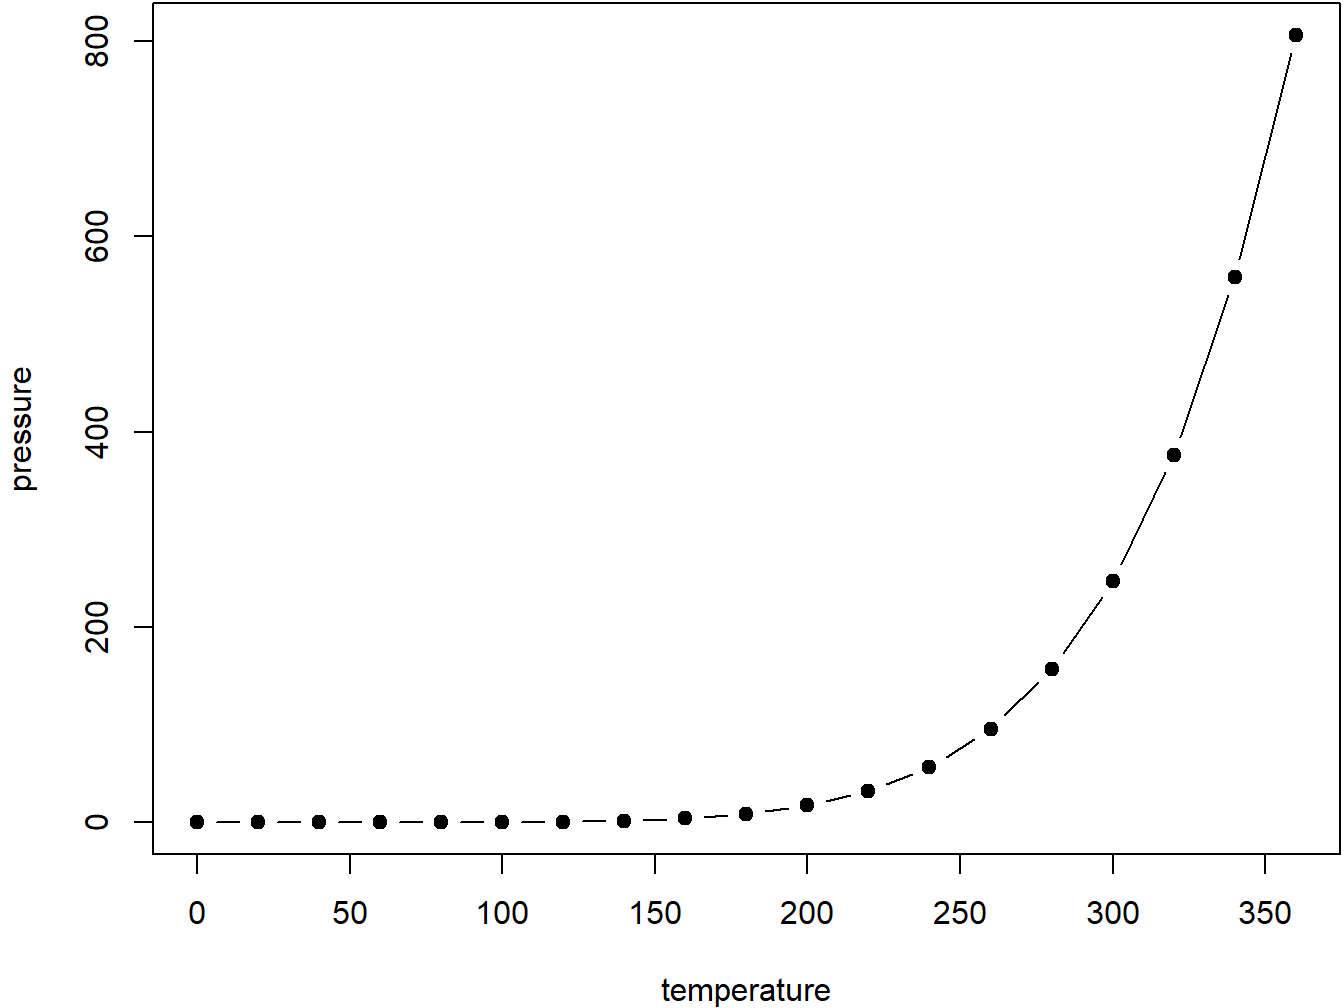
\includegraphics[width=0.8\linewidth]{_main_files/figure-latex/nice-fig-1} 

}

\caption{Here is a nice figure!}\label{fig:nice-fig}
\end{figure}

Don't miss Table \ref{tab:nice-tab}.

\begin{Shaded}
\begin{Highlighting}[]
\NormalTok{knitr}\SpecialCharTok{::}\FunctionTok{kable}\NormalTok{(}
  \FunctionTok{head}\NormalTok{(pressure, }\DecValTok{10}\NormalTok{), }\AttributeTok{caption =} \StringTok{\textquotesingle{}Here is a nice table!\textquotesingle{}}\NormalTok{,}
  \AttributeTok{booktabs =} \ConstantTok{TRUE}
\NormalTok{)}
\end{Highlighting}
\end{Shaded}

\begin{table}

\caption{\label{tab:nice-tab}Here is a nice table!}
\centering
\begin{tabular}[t]{rr}
\toprule
temperature & pressure\\
\midrule
0 & 0.0002\\
20 & 0.0012\\
40 & 0.0060\\
60 & 0.0300\\
80 & 0.0900\\
\addlinespace
100 & 0.2700\\
120 & 0.7500\\
140 & 1.8500\\
160 & 4.2000\\
180 & 8.8000\\
\bottomrule
\end{tabular}
\end{table}

\hypertarget{footnotes}{%
\section{Footnotes}\label{footnotes}}

Footnotes are put inside the square brackets after a caret \texttt{\^{}{[}{]}}. Like this one \footnote{This is a footnote.}.

\hypertarget{citations}{%
\section{Citations}\label{citations}}

Reference items in your bibliography file(s) using \texttt{@key}.

For example, we are using the \textbf{bookdown} package \citep{R-bookdown} (check out the last code chunk in index.Rmd to see how this citation key was added) in this sample book, which was built on top of R Markdown and \textbf{knitr} \citep{xie2015} (this citation was added manually in an external file book.bib).
Note that the \texttt{.bib} files need to be listed in the index.Rmd with the YAML \texttt{bibliography} key.

The RStudio Visual Markdown Editor can also make it easier to insert citations: \url{https://rstudio.github.io/visual-markdown-editing/\#/citations}

\hypertarget{equations}{%
\section{Equations}\label{equations}}

Here is an equation.

\begin{equation} 
  f\left(k\right) = \binom{n}{k} p^k\left(1-p\right)^{n-k}
  \label{eq:binom}
\end{equation}

You may refer to using \texttt{\textbackslash{}@ref(eq:binom)}, like see Equation \eqref{eq:binom}.

\hypertarget{theorems-and-proofs}{%
\section{Theorems and proofs}\label{theorems-and-proofs}}

Labeled theorems can be referenced in text using \texttt{\textbackslash{}@ref(thm:tri)}, for example, check out this smart theorem \ref{thm:tri}.

\begin{theorem}
\protect\hypertarget{thm:tri}{}\label{thm:tri}For a right triangle, if \(c\) denotes the \emph{length} of the hypotenuse
and \(a\) and \(b\) denote the lengths of the \textbf{other} two sides, we have
\[a^2 + b^2 = c^2\]
\end{theorem}

Read more here \url{https://bookdown.org/yihui/bookdown/markdown-extensions-by-bookdown.html}.

\hypertarget{callout-blocks}{%
\section{Callout blocks}\label{callout-blocks}}

The R Markdown Cookbook provides more help on how to use custom blocks to design your own callouts: \url{https://bookdown.org/yihui/rmarkdown-cookbook/custom-blocks.html}

  \bibliography{book.bib,packages.bib}

\end{document}
